\begin{figure}[H]
\centering

\begin{subfigure}{0.45\textwidth}
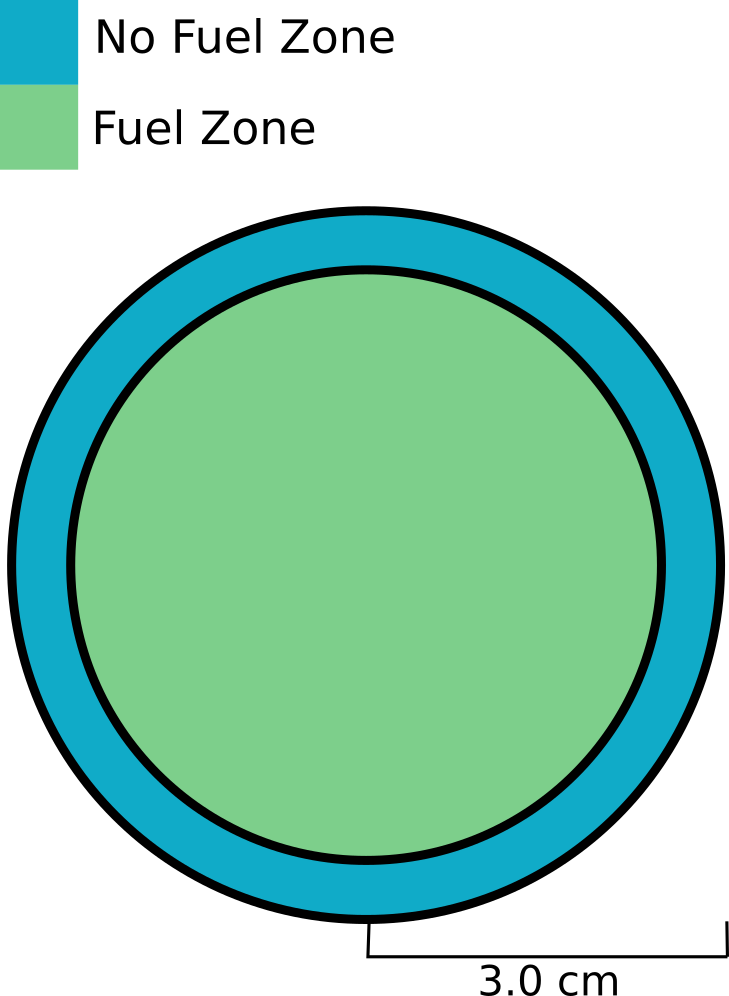
\includegraphics[width=0.9\linewidth]{figures/pebble-zones.png}
\caption{Pebble Zones}
\label{fig:pebb-zone1}
\end{subfigure}%
%
\begin{subfigure}{0.45\textwidth}
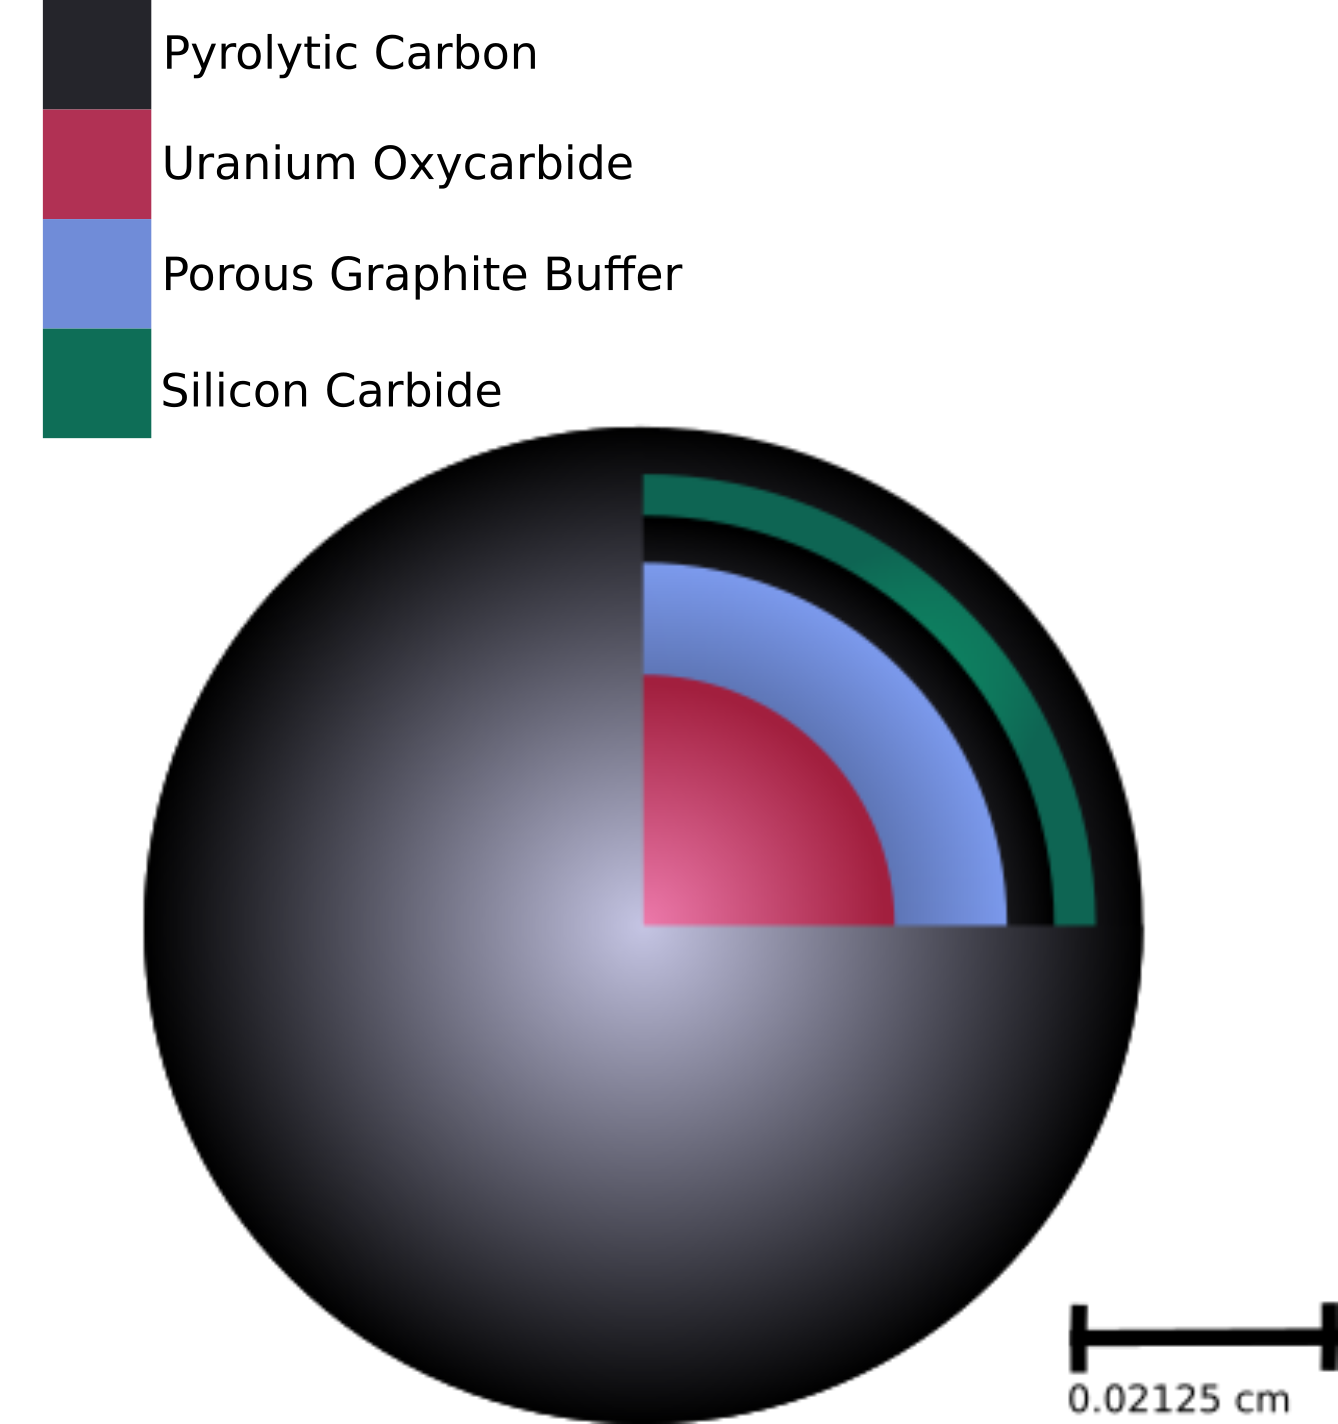
\includegraphics[width=1.1\linewidth]{figures/trisos-r-like-onions.png}
\caption{TRISO Particle Layers}
\label{fig:particle-layer}
\end{subfigure}%

\subfloat[Pebble Parameters]{
\begin{tabular}{ c  c }
\hline
Parameter & Value \\
\hline
Fueled-Center Radius [cm] & 2.5 \\
Graphite Outer Shell Thickness [cm] & 0.5 \\
Total Radius [cm] & 3.0 \\
TRISO Particles per Pebble & 18,000 \\
\hline
\end{tabular}
\label{table:params2}
}
%
\subfloat[Particle Parameters]{
\begin{tabular}{ c  c }
\hline
Parameter & Value [cm] \\
\hline 
Uranium Oxycarbide Kernel Radius & 0.02125 \\
Graphite Layer Thickness & 0.03075 \\
Inner Pyrolytic Carbon Layer Thickness & 0.03475 \\
Silicon Carbide Layer Thickness & 0.03825 \\
Outer Pyrolytic Carbon Layer Thickness & 0.04225 \\
\hline
\end{tabular}
\label{table:params3}
}

\end{figure}
